\chapter{Introduction}
\label{ch:intro}

%\section{Background}
%\label{s:background}

The notion of describing amorphous materials as random networks dates back to \zach, who in 1932 sketched a simple diagram of a \td{} glass \cite{Zachariasen1932}.
This configuration, reproduced in figure \ref{fig:zach_orig}, showed a collection of percolating rings with an absence of long\--range order.
At the time, \zach's image was intended only as schematic to illustrate the analogous effects in \thd{} glasses.
However, some eighty years later, modern synthesis techniques have led to a range of \td{} materials including amorphous carbon, silica and germania which can be considered realisations of \zach's glass \cite{Kotakoski2011,Robertson2012,Huang2012,Lichtenstein2012a,Shaikhutdinov2013,Lewandowski2018,Lewandowski2019}.
These advances may yet represent a watershed moment in chemistry, facilitating the development of a wide range of technologically useful materials with applications including catalysis and gas separation \cite{Trogadas2014,Sun2015a,Buchner2017}.

It is clear that understanding the structure of amorphous materials is key to this aim.
However, due to the relative recentness of these experimental discoveries, much of the existing theory arises from studies of systems on greater length scales.
Specifically, in the second half of the 20\th{} century, much work was carried out on the formation of polycrystals in metals and alloys.
By annealing the metal and slicing through the sample, the grains in the polycrystal could be directly imaged; revealing a system of tessellating polygons not dissimilar to an atomic material \cite{Beck1954,Dunn1957}.

Over time it became apparent that the structure of these networks is constrained on a series of different levels.
Firstly the mean ring size (\ie{} the average number of sides in a polygon) tends to the constant value of six.
This is readily explainable via graph theoretic arguments, resulting from Euler's formula when each vertex forms part of three edges - as is the case for trivalent atoms or the meeting of three grain boundaries.
This is consistent with chemical intuition: a pristine graphene sheet is a hexagonal net and although a Stone\--Wales defect introduces pentagons and heptagons, they occur in pairs to preserve the overall mean ring size \cite{Stone1986}.

The next level of information is then the explicit distribution of polygon sizes, also known as the ring statistics.
With the constraint of a fixed mean, the ring statistics were shown to be relatively well defined, following a lognormal or maximum entropy distribution \cite{Shackelford1981,Lemaitre1993,Lichtenstein2012}.
However, the ring statistics alone are not sufficient to fully describe the network topology. 
This is because the same set of rings can be arranged in a large number of different ways.
Consider again \zach's original configuration. 
Removing one square achieves a mean ring size of six and allows the constituent rings to be arranged as a periodic tiling.
Figures \ref{fig:zach_high}\--\ref{fig:zach_low} show three such examples tilings.


\begin{figure}[h]
     \centering
     
     \begin{subfigure}[b]{0.25\textwidth}
         \centering
         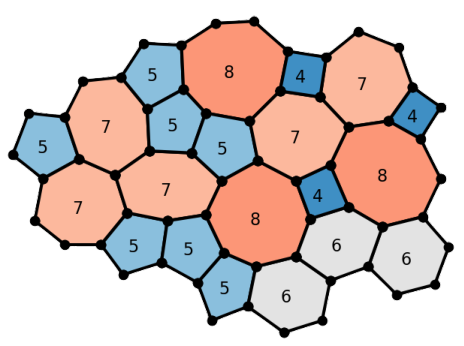
\includegraphics[width=\textwidth]{./figures/introduction/zach_orig.pdf}
         \caption{}
         \label{fig:zach_orig}
     \end{subfigure}
     \hspace{1cm}
     \begin{subfigure}[b]{0.25\textwidth}
         \centering
         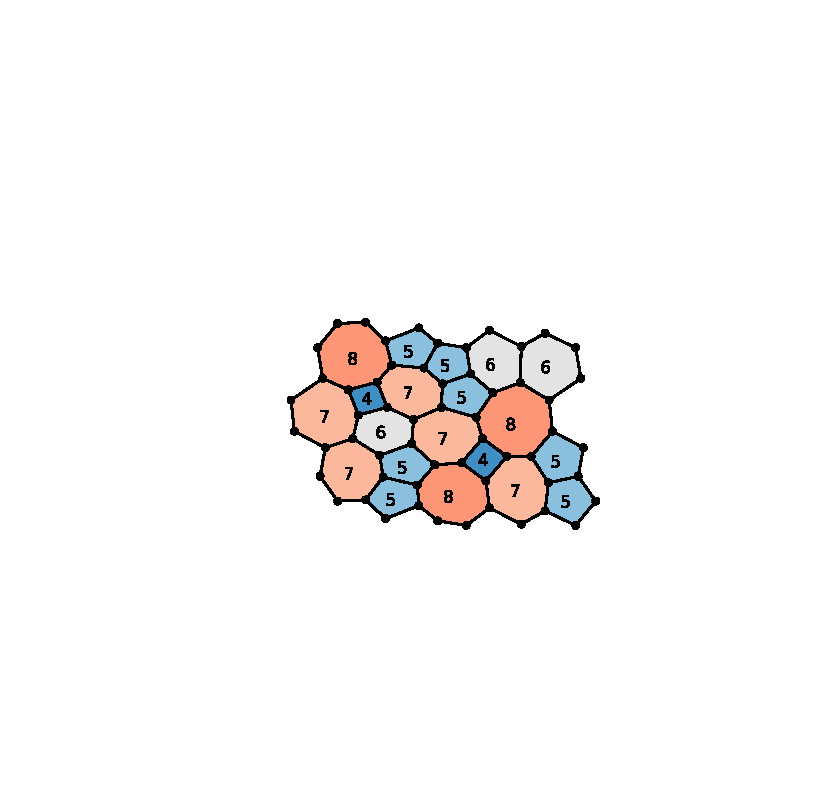
\includegraphics[width=\textwidth]{./figures/introduction/zach_high.pdf}
         \caption{}
         \label{fig:zach_high}
     \end{subfigure}
     
     \begin{subfigure}[b]{0.25\textwidth}
         \centering
         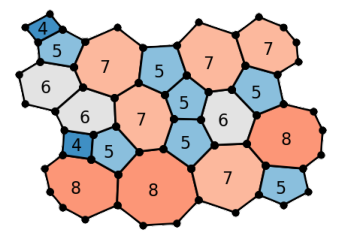
\includegraphics[width=\textwidth]{./figures/introduction/zach_mid.pdf}
         \caption{}
     \end{subfigure}
     \hspace{1cm}
     \begin{subfigure}[b]{0.25\textwidth}
         \centering
         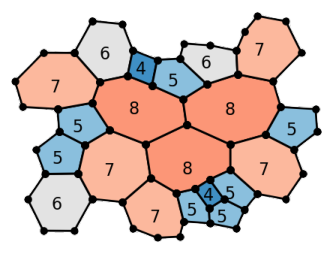
\includegraphics[width=\textwidth]{./figures/introduction/zach_low.pdf}
         \caption{}
         \label{fig:zach_low}
     \end{subfigure}
     
     \caption{Panel (a) shows \zach's glass and panels (b)\--(d) three different periodic arrangements based on the glass (with one square removed to satisfy Euler's formula). Moving from panel (b)\--(d) there is increased clustering of similar sized rings. The size of the rings are highlighted numerically and by colour.}
     \label{fig:zach}
\end{figure}

Whilst they may initially look similar, on closer inspection the three configurations display fundamentally different properties.
In figure \ref{fig:zach_high} similar sized rings are dispersed throughout the arrangement whilst in \ref{fig:zach_low} they are tightly clustered together.
Furthermore, given the large number of configurations which may be theoretically possible for any set of ring statistics, only a subset of these may be physically realisable.
Empirically, these are found to be the ones in which large rings tend to be surrounded by smaller rings \ie{} similar to \ref{fig:zach_high}.
Once again, chemical intuition would support this in the context of atomic materials, as strain is minimised by maintaining bond lengths and angles as close to their equilibrium values as possible.
This effect was first noticed in polycrystals and quantified through the \aw{} law \cite{Aboav1970,Weaire1974}.
This law posits that the mean ring size about any given ring can be related to the central ring size by a single fitting parameter.
Hence the value of this parameter in some way describes the increased tendency of the small rings to be adjacent to large rings.
The \aw{} parameter therefore provides information on the first\--order ring correlations, completing the topological description of the network material.

The novelty and potential usefulness of \td{} materials makes them a  clear candidate for computational study, in order to complement and supplement experimental endeavours. 
Taking the example of thin silica films, there have already been multiple complementary computational investigations including both \abinitio{} methods and molecular dynamics studies using classical force fields at varying levels of theory \cite{Bjorkman2013,Malashevich2016,Wilson2013,Wilson2018,Zhang2018a,Bamer2019,Roy2019,Richter2019}.
In order to perform these simulations, it is necessary to have a starting atomistic configuration.
This can be achieved in multiple ways. 
The most straightforward is to take one of the existing experimental images. 
These are however limited in size and number and can contain defects or areas which cannot be fully imaged.
In addition, some related experimental systems have proved significantly more challenging to synthesise, such as bilayers of germania \cite{Lewandowski2018,Lewandowski2019}.
As a result, computational techniques are often preferable, but generating configurations will the required topological properties (\ie{} correct ring statistics \textit{and} \aw{} parameter) has proved surprisingly difficult \cite{Roy2018,Kumar2014}.
Therefore, the first part of this thesis will focus on developing methods to generate configurations of \td{} networks in which the topological parameters can be tuned in a controllable manner.
These configurations can then be used as a seed for further computational studies, removing some of the reliance on experimental configurations and opening the door for high\--throughput calculations which can be speculative and potentially predictive.

However, the scope of this work extends beyond materials modelling.
As previously mentioned, much of the original work in this field focussed on polycrystals of metal oxides with some links to foams and Voronoi polygons \cite{Aboav1980,Boots1984}.
It is now clear that these chemical networks fit into a much wider class of \td{} physical networks that are ubiquitous in the natural world, emerging across physical disciplines and length scales.
Traditional examples range from the atomic level of ultra\--thin materials, through colloids, foams, epithelial cells and all the way to geological rock formations \cite{Earnshaw1994,Allain1995,Moncho-Jorda2000,Durand2011,Tong2017,Goehring2014}.
There are however countless more occurrences, with drying blood, stratocumulus clouds, crocodile scales and geopolitical borders all being the subject of studies \cite{Brutin2011,Glassmeier2017,Milinkovitch2019,LeCaer1993}.
More intriguingly, although these systems are incredibly physically diverse, they have strikingly similar structures \cite{Schliecker1999}. 
This is because they can all be mapped onto the same generic system, which can be equivalently described as a collection of tessellating polygons or percolating rings, and hence they are governed by the same fundamental laws. 
Understanding the behaviours of \td{} networks is therefore key to a wide range of problems in frontier research, not only the directed synthesis of nano\--materials but also for example the control of mitotic division \cite{Gibson2011,Ladan2019}; as well as to curiosities such as explaining the arrangement of the stones in Giant's Causeway or cracking in famous artworks \cite{Weaire1984,Flores2017}.

Coupled with these observations, the continuing expansion and maturity of network science as a field has led to significant advances in the description and characterisation of complex networks.
This has largely been driven by interest in networks in the more abstract sense of the internet, social media and neural networks \cite{Strogatz2001,Boccaletti2006,Barabasi2012}.
To date, the application of these principles in the physical sciences has mostly been confined to topics such as biological signalling pathways.
The second part of this thesis will therefore show how robust metrics from network science can be applied to physical \td{} networks to better quantify their structure and replace the need for empirical measures such as the \aw{} law.
As part of this process, more generic methods are developed to construct \td{} networks across a range of potential models, coordination environments and topologies.
This allows a systematic study into the factors which influence the underlying network properties in \td{} systems.
More broadly, this has the effect of tying physical \td{} networks into the wider field of network science, showing them to be a unique and interesting addition to the area.

The later parts of this thesis will apply the developed concepts and techniques to a series of related and novel problems across chemistry.
To given a broad overview, this will begin with an investigation into the network analysis of quasi\--two\--dimensional hard sphere systems, which is of direct relevance to on\--going experimental studies of colloidal monolayers \cite{Thorneywork2017}.
In such systems, the ring structure emerges through construction of a Voronoi diagram, which partitions the sample space into polygonal regions associated with each particle.
Whilst the properties of Voronoi diagrams are well understood for two\-- and three\--dimensional systems, the intermediate dimensionality of colloidal monolayers leads to novel challenges in their characterisation.
Following this, attention will be turned to another system of relatively recent interest, that of ``procrystalline'' lattices \cite{Overy2016}.
These procrystals can also be considered to have intermediary behaviour, in that they have atoms located on a regular, ordered lattice and yet have disordered ring structure - hence lying between the crystalline and amorphous states.
This partial ordering raises the possibility of procrystals displaying fundamentally different behaviour, in terms of their network properties, to either crystalline or amorphous materials.
Finally, a new tool from topological data analysis, termed persistent homology, will be applied to \td{} amorphous materials.
The aim of persistent homology is to find the fundamental topological features in generic point sets, and so holds the potential to identify and characterise the ring structure in atomic networks \cite{Wasserman2018}.
Although the method is in its relative infancy, the effectiveness of persistent homology in quantifying disorder in the case of \td{} materials can be examined ahead of time through the use of computational models.
\davidnote{Is this paragraph all too brief or about right?}

These interrelated examples raise two important questions central to this work, namely why is the focus on \td{} systems, and why on computational modelling?
To answer the first of these questions, one may argue it is precisely because there exist experimental realisations of quasi\--two\--dimensional systems, which have a range of technologically useful applications \cite{Butler2013,Bhimanapati2015,Tan2017}.
Alternatively, it may be said that a \td{} system is in some way a simplified version of a \thd{} assembly, and so they provide a tractable way of studying the behaviours of higher dimensionality systems.
Whilst both these statements have merit, neither is entirely satisfactory, as the former neglects to explain why such experiments are successful and latter is not universally true \cite{ChaikinPaulM1995}.
Two\--dimensional systems can display their own unique constraints, which in fact often leads to the desirable properties of nanomaterials.
What study in two dimensions provides, is the opportunity to visualise, analyse and understand systems which are inherently more tangible.
Raw data is available experimentally in real\--space, without the need for transformation, as required with structure factors or diffraction patterns.
From this data, metrics such as the ring structure is well defined and readily extractable.
This in turn allows the development of simulation and analysis methods which are able to accurately model and characterise the system, and leads to a more complete understanding.
It is then the ideal that the insight gained can be applied to higher dimensions, or used to aid the synthesis of materials with analogous properties.
\davidnote{Is this paragraph pointless waffle?}

In response to the second question, the power of computational modelling as complement to experiment arises from the ability to reproduce experimental results, but also explore experimentally inaccessible systems.
As previously mentioned, experimental data, such as STM, from frontier research is difficult to produce and may be incomplete or relatively small in extent.
Computational models can help to fill any gaps and provide information as to the frequency or stability of the observed sample.
Moreover, computation has access to a greater number of observables than experiment, which can provide explanation for a given phenomenon.
Finally, and perhaps most importantly, simulation allows a holistic study of materials by continuously varying parameters to generate structures which may or may not map onto those from experiment.
This enables properties to systematically explored, in principle leading to the holy grail of computational modelling, that of predictive capability.
This thesis aims to incorporate all of these aspects, designing models and algorithms to simulate a wide range of \td{} systems, developing metrics to better characterise them and compare to experiment, and ultimately pushing these models outside the current experimental bounds.  
\davidnote{As above?}
\davidnote{Revisit intro to make more consistent with conclusion and include reiterate key themes of work}

%\section{Thesis Structure}
%
%The structure of this thesis is as follows:
%\davidnote{Todo: thesis structure}
%\davidnote{Just basically a repeat of abstracts?}
%\davidnote{Actually can this section just go?}
%
%\begin{itemize}
%	\item \textbf{Chapter 2}: the theory underpinning complex networks is discussed, covering the representation of atomic systems as networks and the relationship of the dual network to ring structure.
%The laws which govern the topological properties of physical networks are also introduced, namely Euler's law, \lm's law and the \aw{} law.
%
%	\item \textbf{Chapter 3}: the theoretical basis of \mc{} methods and their application to generating realisations of \td{} networks is reviewed.
%There is a broad discussion of Metropolis \mc{} methods, before specific methods are covered in detail; namely the bond switching algorithm and hard particle \mc{} in conjunction with the Voronoi construction.
%This discussion lays the groundwork for the extension of these methods and development of additional \mc{} algorithms in subsequent chapters.
%	
%	\item \textbf{Chapter 4}: a computationally tractable \mc{} method using triangle rafts is developed to generate bilayers of \sioii{} and related materials.
%The method allows defect free networks of any given shape to be grown with both tuneable ring statistics and topologies, controlled by a combination of the choice of the ``allowed'' rings and the effective growth ``temperature''. 
%Configurations are generated with \aw{} parameters commensurate with those obtained from an analysis of experimental configurations, improving significantly on previous methods.
%The ability to efficiently grow configurations allows exploration of the structural basis of \lm’s law, where the commonly observed value of $p_6\approx0.4$ is presented as a balance between entropic and enthalpic factors. 
%The deviations of ring areas from the ideal values are discussed and the relative insensitivity of the ring area to relatively strong distortions is highlighted.
%	
%	\item \textbf{Chapter 5}:
%	
%	\item \textbf{Chapter 6}:
%	
%	\item \textbf{Chapter 7}:
%	
%	\item \textbf{Chapter 8}:
%
%	\item \textbf{Chapter 9}:
%	
%	\item \textbf{Chapter 10}:
%\end{itemize}
	
 
